\solutionset

\begin{enumerate}

\item \textbf{HII Region Trapping.}

\begin{enumerate}

\item The density profile of the accretion flow is given implicitly by
\begin{displaymath}
\dot{M}_* = 4\pi r^2 \rho v_{\rm ff},
\end{displaymath}
where $v_{\rm ff} = \sqrt{2 G M_*/r}$. Thus we have
\begin{displaymath}
\rho = \frac{\dot{M}_*}{4\pi \sqrt{2G M_*}} r^{-3/2}.
\end{displaymath}
Recombinations happen in the region between $R_*$ and $r_i$. The recombination rate per unit volume is $\alpha_B n_e n_p = 1.1 \alpha_B (\rho/\mu_{\rm H})^2$, where $\mu_{\rm H} =2.3\times 10^{-24}$ g is the mass per H nucleus assuming standard composition. Thus the total recombination rate within the ionized volume is
\begin{eqnarray*}
\Gamma & = & \int_{R_*}^{r_i} 4\pi r^2 (1.1\alpha_B) \left(\frac{\dot{M}_*}{4\pi \mu_{\rm H} \sqrt{2G M_*}} r^{-3/2}\right)^2 \, dr \\
& = & \frac{1.1\alpha_B \dot{M}_*^2}{8\pi \mu_{\rm H}^2 G M_*} \ln \frac{r_i}{R_*}.
\end{eqnarray*}
Since this must equal the ionizing photon production rate ($\Gamma = S$), we can solve for $r_i$:
\begin{displaymath}
r_i = R_* \exp\left(\frac{8\pi \mu_{\rm H}^2 G M_* S}{1.1 \alpha_B \dot{M}_*^2}\right).
\end{displaymath}
The condition that $r_i \gg R_*$ is satisfied if the term inside parentheses is $\gtrsim 1$, which in turn requires
\begin{displaymath}
\dot{M}_* \lesssim \left(\frac{8\pi \mu_{\rm H}^2 G M_* S}{1.1 \alpha_B}\right)^{1/2}.
\end{displaymath}
Plugging in the given values $M_* = 30$ $\msun$ and $S=10^{49}$ s$^{-1}$, we obtain $\dot{M}_* \lesssim 7\times 10^{-5}$ $\msun$ yr$^{-1}$. This is lower (though not by a huge amount) than the typical accretion rates inferred for massive stars.

\item The escape velocity at a distance $r$ from the star is $v_{\rm esc} = \sqrt{2 G M_*/r}$. Thus the condition that $v_{\rm esc} < c_i$ at $r_i$ implies that
\begin{displaymath}
\frac{2 G M_*}{c_i^2} <  r_i = R_* \exp\left(\frac{8\pi \mu_{\rm H}^2 G M_* S}{1.1 \alpha_B \dot{M}_*^2}\right).
\end{displaymath}
Solving for $\dot{M}_*$, we find
\begin{displaymath}
\dot{M}_* > \left[\frac{8\pi \mu_{\rm H}^2 G M_* S}{2.2\alpha_B \ln(v_{\rm esc,*}/c_i)}\right]^{1/2},
\end{displaymath}
where $v_{\rm esc,*} = \sqrt{2 G M_*/R_*}$ is the escape speed from the stellar surface. Using $R_*=7.7$ $\rsun$ (the radius of a 30 $\msun$ ZAMS star) and plugging in the other input values gives $\dot{M}_*>2.2\times 10^{-5}$ $\msun$.

\end{enumerate}

\item \textbf{The Transition to Grain-Mediated H$_2$ Formation}\footnote{This problem was primarily inspired by \citet{glover03a}.}

\begin{enumerate}

\item To calculate the rate of H$_2$ formation catalyzed by free electrons, we first calculate the rate of formation of H$^-$:
\begin{displaymath}
\gamma({\rm H}^{-}\,{\rm form.}) = k_{-} n_e n_{\rm H} = k_{-} x_{\rm C} Z n_{\rm H}^2,
\end{displaymath}
where $k_{-} = 1.1\times 10^{-16} T_2^{0.88}$ cm$^3$ s$^{-1}$ is the rate coefficient given in Chapter \ref{ch:first_stars}. Next we must calculate the fraction of H$^-$ ions formed that yield H$_2$. The H$^-$ can be destroyed either by photodetachment or by reacting with a neutral hydrogen to form H$_2$:
\begin{displaymath}
{\rm H}^{-} + {\rm H} \rightarrow {\rm H}_2 + e^{-}.
\end{displaymath}
The rate of the latter reaction is
\begin{displaymath}
\gamma({\rm H}^{-}\rightarrow{\rm H}_2) = k_2 n_{{\rm H}^-} n_{\rm H}
\end{displaymath}
with $k_2 = 1.3\times 10^{-9}$ cm$^3$ s$^{-1}$ (the value given in class). The rate of photodetachment is
\begin{displaymath}
\gamma({\rm H}^{-}\,{\rm photo.}) = \zeta_{\rm pd} n_{{\rm H}^-}
\end{displaymath}
with $\zeta_{\rm pd} = 2.4\times 10^{-7}$ s$^{-1}$ for the Milky Way radiation field, again as given in class. Thus the branching ratio for H$^{-}$ going to H$_2$ rather than being destroyed by photodetachment is
\begin{displaymath}
\Gamma({\rm H}^{-}\rightarrow{\rm H}_2) = \frac{\gamma({\rm H}^{-}\rightarrow{\rm H}_2)}{\gamma({\rm H}^{-}\rightarrow{\rm H}_2) + \gamma({\rm H}^{-}\,{\rm photo.})} = \frac{k_2 n_{\rm H}}{k_2 n_{\rm H}+\zeta_{\rm pd}}
\end{displaymath}
Putting this together, the rate of formation of H$_2$ via free electrons is
\begin{eqnarray*}
\gamma({\rm H}_2{\rm - gas}) & = & \gamma({\rm H}^{-}\,{\rm form.}) \Gamma({\rm H}^{-}\rightarrow{\rm H}_2) \\
& = & k_{-} x_{\rm C} Z  \left[1+ \zeta_{\rm pd}/(k_2 n_{\rm H})\right]^{-1} n_{\rm H}^2. 
\end{eqnarray*}
In comparison, the rate of H$_2$ formation on grain surfaces is simply
\begin{displaymath}
\gamma({\rm H}_2{\rm - grain}) = R n_{\rm H}^2 = R_{\odot} Z n_{\rm H}^2,
\end{displaymath}
where $R_{\odot} = 3\times 10^{-17}$ cm$^3$ s$^{-1}$ is the rate coefficient at Solar metallicity. Taking the ratio of these two, we have
\begin{eqnarray*}
\frac{\gamma({\rm H}_2{\rm - grain})}{\gamma({\rm H}_2{\rm - gas})} & = & \frac{R_{\odot} \left[1+ \zeta_{\rm pd}/(k_2 n_{\rm H})\right]}{k_{-} x_{\rm C}} \\
& = & 2700 T_2^{-0.88} \left[1+ \zeta_{\rm pd}/(k_2 n_{\rm H})\right].
\end{eqnarray*}
Thus even in the limit $n_{\rm H} \rightarrow \infty$, the rate of formation on grain surfaces exceeds that in the gas phase by $\sim 3$ orders of magnitude. At densities below $\zeta_{\rm pd}/k_2 = 185$ cm$^{-3}$, where photodetachment significantly inhibits H$_2$ formation via the H$^-$ channel, grain formation wins by an even larger factor.\\

\item For gas phase formation, this calculation is exactly the same as the previous part, with two minor differences. First, the factor $x_{\rm C} Z$ in the gas-phase formation rate is replaced by $x$, since how hydrogen rather than carbon is the dominant source of free electrons. Second, all the $n_{\rm H}$ factors become $(1-x) n_{\rm H}$, since only neutral hydrogen participates in the relevant reactions. Making these changes, the H$^-$ formation rate is
\begin{displaymath}
\gamma({\rm H}^{-}\,{\rm form.}) = k_{-} x (1-x) n_{\rm H}^2,
\end{displaymath}
and the H$^-$ to H$_2$ reaction rate is
\begin{displaymath}
\gamma({\rm H}^{-}\rightarrow{\rm H}_2) = k_2 (1-x) n_{{\rm H}^-} n_{\rm H}.
\end{displaymath}
The photodetachment rate is unchanged, so the branching ratio for H$^-$ going to H$_2$ becomes
\begin{displaymath}
\Gamma({\rm H}^{-}\rightarrow{\rm H}_2) = \frac{k_2 (1-x) n_{\rm H}}{k_2 (1-x) n_{\rm H}+\zeta_{\rm pd}},
\end{displaymath}
and the gas-phase H$_2$ formation rate is therefore
\begin{displaymath}
\gamma({\rm H}_2{\rm - gas}) = k_{-} x (1-x)  \left[1+ \zeta_{\rm pd}/(k_2 (1-x) n_{\rm H})\right]^{-1} n_{\rm H}^2. 
\end{displaymath}
The grain-mediated reaction rate becomes
\begin{displaymath}
\gamma({\rm H}_2{\rm - grain}) = R_{\odot} Z (1-x) n_{\rm H}^2.
\end{displaymath}
Notice that there is only one factor of $x$, because the reaction rate involves the collision of neutral hydrogen atoms with dust grains, and therefore depends on the density of gas times the density of grains. If the ionization fraction is $x$, the neutral hydrogen fraction is reduced by a factor $(1-x)$, but the grain abundance is unchanged. Setting the two rates equal, we have
\begin{displaymath}
k_{-} x \left[1+ \zeta_{\rm pd}/(k_2 (1-x) n_{\rm H})\right]^{-1} = R_{\odot} Z.
\end{displaymath}
This is a quadratic in $x$, and the solution is
\begin{displaymath}
x = \frac{1}{2}\left(1+k \pm \sqrt{1-2k + k^2 - 4 k/r_{\rm pd}}\right)
\end{displaymath}
\begin{marginfigure}
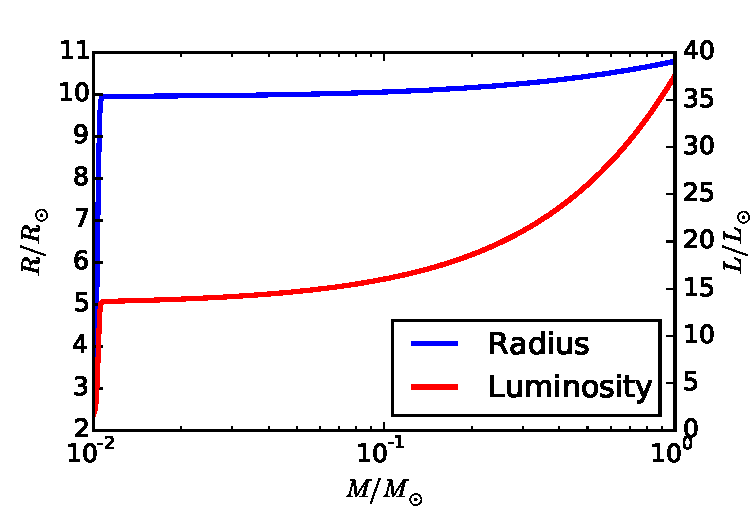
\includegraphics[width=\linewidth]{hw5sol1}
\caption[Solution to problem set~\thesolutionset, problem~\theenumi\theenumii]{
\label{fig:hw5sol1}
$x$ versus $Z$ for $n_{\rm H} = 1$, 10, and 100 cm$^{-3}$.
}
\end{marginfigure}
where $k = R_{\odot} Z/k_{-}\approx 0.27 T_2^{-0.88} Z$ is the ratio of the rate coefficients for H$_2$ formation on grains and H$^-$ formation in the gas phase, and $r_{\rm pd} = n_{\rm H} k_2 / \zeta_{\rm pd}$ is the ratio of the gas density to the critical density for H$_2$ photodetachment, $n_{\rm crit,pd} = \zeta_{\rm pd}/k_2\approx 185$ cm$^{-3}$. Note that both roots represent mathematically valid solutions, one at ionization fraction below 50\% and one at ionization fraction above 50\%. In practice, however, the low ionization fraction solution is the more physically-realistic one, since if the gas is highly ionized the temperature is unlikely to be low enough to allow formation of H$_2$. Figure \ref{fig:hw5sol1} shows the physically-realistic solution plotted for $n_{\rm H} = 1$, 10, and 100 cm$^{-3}$.

\item A solution ceases to exist when the metallicity is such that the quantity under the square root in the equation from the previous part goes to zero. Thus, grain-mediated H$_2$ formation must dominate whenever
\begin{displaymath}
1 - 2k + k^2 - 4 k r_{\rm pd}^{-1} < 0.
\end{displaymath}
Solving, this condition reduces to
\begin{displaymath}
k > 1 + \frac{2}{r_{\rm pd}} \left(1 - \sqrt{1+r_{\rm pd}}\right).
\end{displaymath}
(Note: there is another root to this equation, with a $+$ instead of a $-$ in front of the square root. However, one can easily verify that in the vicinity of this root $x>1$, which is obviously unphysical. Thus the $-$ root is the physically realistic one.) Rewriting this in terms of dimensional quantities, this is
\begin{marginfigure}
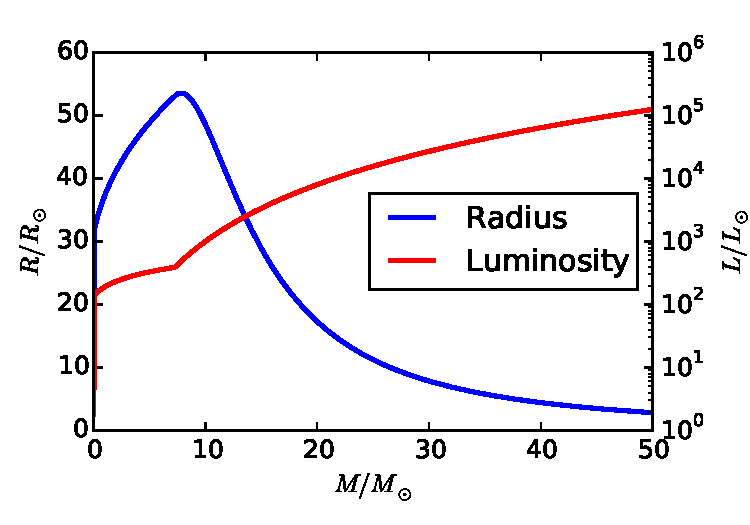
\includegraphics[width=\linewidth]{hw5sol2}
\caption[Solution to problem set~\thesolutionset, problem~\theenumi\theenumii]{
\label{fig:hw5sol2}
$Z$ versus $n_{\rm H}$ at $T=100$ K and $1000$ K.
}
\end{marginfigure}
\begin{displaymath}
Z > 0.27 T_2^{0.88} \left[1 + \frac{2 n_{\rm crit,pd}}{n_{\rm H}} \left(1 - \sqrt{1+\frac{n_{\rm H}}{n_{\rm crit,pd}}}\right)\right].
\end{displaymath}
Figure \ref{fig:hw5sol2} shows a plot of the minimum value of $Z$ versus density $n_{\rm H}$ at $T=100$ K and 1000 K.

\end{enumerate}


\item {\bf Disk Dispersal by Photoionization.}

\begin{enumerate}

\item The gas will escape when the sound speed becomes comparable to the escape speed from the star. Thus
\begin{eqnarray*}
c_s & \approx & \sqrt{\frac{2 G M_*}{r_g}}\\
r_g & \approx & \frac{2 G M_*}{c_s^2} = \frac{2 G M_* \mu}{k_B T}
\end{eqnarray*}
The mean particle mass depends on whether the helium is ionized or not, but for a relatively cool star like a T Tauri star it is probably reasonable to assume that it is not, so the number of electrons equals the number of hydrogen atoms. The mean mass per particle for neutral hydrogen is $2.34\times 10^{-24}$ g, and by number hydrogen represents 93\% of all nuclei in the Milky Way, so the mean mass per particle in gas where the hydrogen is ionized is $\mu=1.2\times 10^{-24}$ g. Plugging this in gives a sound speed $c_s = 10.7$ km s$^{-1}$.

\item Ionization balance requires that recombinations equal ionizations. If the density is $n_0$ inside $r_g$, the recombination rate per unit volume is $\alpha^{(B)} n_0^2$, where $\alpha^{(B)}=2.59\times 10^{-13}$ cm$^{-3}$ s$^{-1}$ is the case B recombination coefficient, and this expression implicitly assumes that the gas is fully ionized. The recombination rate is simply this times the volume, so equating this with the ionization rate produced by the star give
\begin{eqnarray*}
\Phi & = & \frac{4}{3}\pi r_g^3 \alpha^{(B)} n_0^2 \\
n_0 & = & \sqrt{\frac{3\Phi}{4\pi \alpha^{(B)} r_g^3}} \\
& = & \sqrt{\frac{3\Phi k_B^3 T^3}{32\pi \alpha^{(B)} G^3 M_*^3 \mu^3}}
\end{eqnarray*}

\item The wind will have a density of $\sim n_0$ and will leave a velocity $\sim c_s$, and it will be lost from an area of order $r_g^2$. Thus an order of magnitude estimate for the wind mass flux is
\begin{eqnarray*}
\dot{M} & \sim & n_0 m_H c_s r_g^2 \\
& = & \sqrt{\frac{3\Phi r_g}{4\pi \alpha^{(B)}}} m_H c_s \\
& = & \sqrt{\frac{3\Phi G M_* m_H^2}{2\pi \alpha^{(B)}}}
\end{eqnarray*}

\item Plugging in the given numerical values gives $\dot{M} \sim 10^{-10}$ $\msun$ yr$^{-1}$. Thus it would take $\sim 100$ Myr to evaporate a $0.01$ $\msun$ star. This is much longer than the observed $\sim 2$ Myr lifetime of T Tauri disks. This indicates that photoionization by itself cannot the the primary disk removal mechanism. Instead, it is a plausible disk destruction mechanism only if it operates in tandem with some other mechanism, like accretion of the disk onto the star.

\end{enumerate}

\item {\bf Aerodynamics of Small Solids in a Disk.}

\begin{enumerate}

\item The force per unit mass in the radial direction that a parcel of gas of density $\rho$ experiences due to the combined effects of gas pressure and stellar gravity is
\begin{displaymath}
f_r = -\frac{G M}{r^2} - \frac{1}{\rho}\frac{\partial P}{\partial r} = -\frac{GM}{r^2} + \frac{n}{\rho}\frac{P}{r} = -\frac{GM}{r^2} + \frac{n c_s^2}{r}.
\end{displaymath}
This also gives the acceleration of the gas parcel toward the star. If we equate this with the centripetal acceleration required to maintain circular motion at velocity $v_g$, then we have
\begin{displaymath}
\frac{v_g^2}{r} = \frac{GM}{r^2} - \frac{n c_s^2}{r} = \frac{v_K^2}{r} - \frac{n c_s^2}{r},
\end{displaymath}
where $v_K = \sqrt{GM/r}$ is the Keplerian velocity. If we solve this for $v_g$ and subtract the result from $v_K$, then we have
\begin{eqnarray*}
\Delta v = v_K - v_g & = & v_K - \sqrt{v_K^2 - n c_s^2} \\
& = & v_K \left(1 - \sqrt{1 - \frac{n c_s^2}{v_K^2}}\right) \\
& \approx & \frac{n c_s^2}{2 v_K^2},
\end{eqnarray*}
where the last step results from taking the Taylor expansion of the square root term in the limit $nc_s^2 \ll v_K^2$, which is equivalent to the assumption that the deviation from Keplerian rotation is small.

\item The mass of the solid particle is $m_s = (4/3)\pi s^3 \rho_s$, so its momentum is $p = (4/3)\pi s^3 \rho_s v$. Dividing this by the drag force we have
\begin{displaymath}
t_s = \frac{p}{F_D} = \frac{s}{c_s}\frac{\rho_s}{\rho_d}.
\end{displaymath}
i.e.\ the stopping time is just the sound crossing time of the particle's radius multiplied by the ratio of solid density to gas density.

\item In the frame co-rotating with the gas, the dust particle experiences a net radial force which contains contributions from inward stellar gravity, outward centrifugal force, and outward drag force resisting inward motion. The total force is
\begin{eqnarray*}
F & = & -\frac{GM m_s}{r^2} + \frac{m_s v_g^2}{r} - \frac{4\pi}{3} s^2 \rho_d v c_s \\
& = & -\frac{v_K^2}{r} m_s + \left(\frac{v_K^2}{r} - \frac{n c_s^2}{r}\right) m_d - \frac{4\pi}{3} s^2 \rho_d v c_s \\
& = & \frac{c_s}{m_s} \left(-\frac{nc_s}{r} - \frac{v}{s}\frac{\rho_d}{\rho_s}\right),
\end{eqnarray*}
where $m_s = (4/3)\pi s^3 \rho_s$ is the mass of the solid. The terminal velocity of the grain is determined by the condition that the net force be zero, so if we set the right-hand side of this equation equal to zero and solve, we find that the terminal velocity is
\begin{displaymath}
v = -n c_s\frac{s}{r} \frac{\rho_s}{\rho_d}.
\end{displaymath}
The time required for the solid particle to drift into the star is roughly
\begin{displaymath}
t_{\rm drift} \approx \frac{r_0}{-v} = \frac{r_0^2}{n c_s s}\frac{\rho_d}{\rho_s},
\end{displaymath}

\item First let's evaluate the stopping time:
\begin{displaymath}
t_s = \frac{s}{c_s} \frac{\rho_s}{\rho_d} = \frac{s}{\sqrt{k_B T/\mu}} \frac{\rho_s}{\rho_d} = 2.1\times 10^4\mbox{ s}.
\end{displaymath}
The orbital period at 1 AU is $t_{\rm orb} = 1\mbox{ yr} = 3.1\times 10^7\mbox{ s}$, so we do have $t_s \ll t_{\rm orb}$. The timescale required for the particle to drift into the star is
\begin{displaymath}
t_{\rm drift} =  \frac{r_0^2}{n c_s s}\frac{\rho_d}{\rho_s} = 1.7\times 10^{11}\mbox{ s} = 5400\mbox{ yr}.
\end{displaymath}
This is much, much smaller than the inferred timescale of $\sim 1$ Myr for planet formation and disk dissipation.

\end{enumerate}

\end{enumerate}



